% !TEX root = 0_main.tex

\section{Theoretical Framework}
\label{sec:theoretical-framework}

Crowdsourcing has many definitions, but can be captured by the idea of an open call for anyone to participate in an online task \cite{brabham2013crowdsourcing, estelles2012towards,howe2008crowdsourcing} by contributing information, knowledge, or skills. The `crowd' refers to the group of people who participate in the crowdsourcing initiative online. The crowd can, in theory, emerge from anyone online or specific subsets of people. Participation is either voluntary (uncompensated) or for money (financially incentivised). An instance of voluntary crowdsourcing can be found in crowdsourced journalism \cite{aitamurto2015motivation} or crowdsourcing in crisis management \cite{schimak2015crowdsourcing}. In paid crowdsourcing, participants are compensated per task, as in microtasking on digital labour market-places such as Amazon Mechanical Turk (AMT) \cite{shank2016using} or based on performance as in innovation challenges \cite{jeppesen2010marginality}.

For this research, we frame our case study as part of the aforementioned broader phenomenon of crowdsourcing. More specifically, we draw on Hansson et al.'s \cite{hansson_capitalizing_2018, hansson_alienation_2017} categorisation of the different modes of production in crowdsourcing platforms to frame AOD as a case of \textit{human computing}.  \textit{Human computing} crowdsourcing platforms, such as Amara and AMT, are those in which ``users do micro-tasks that do not require much expertise, such as transcribing audio and video files, translating texts, or tagging maps [...] [, and in which] individual crowd members usually undertake tasks independently of one another, sometimes even competing for work on this market [...]'' \cite{hansson_capitalizing_2018}. In this study, Hansson et al. \cite{hansson_capitalizing_2018} draw on Marx's \cite{10.2307/2550890} theory of alienation to understand the relationships between participants in crowdsourcing and the role of the platforms employed to mediate in the activities. Marx \cite{10.2307/2550890} described four types of relationships: (1) between producer and consumer, (2) between the producer and product, (3) the producers’ relationship to themselves, and (4) their relationships to other producers. Applying Marx's theory of alienation to crowdsourcing, Hansson et al. \cite{hansson_capitalizing_2018} developed a typology of alienation that reveals significant differences between the cases studied. Figure \ref{fig:hansson_adapted}, adapted from their work, depicts the cases of Amara and AMT. For example, with regards to the relationship between an individual producer with the rest of the producers, the position of Amara being closer towards the inner circle means there are stronger bonds between producers (linguists, in the case of Amara). For the case of AMT, which is in the fourth outer circle, this position represents a lack of bonds between producers. This typology is not to be understood as mutually exclusive: these concepts and different modes sometimes co-exist within the same platforms and processes. However, this typology is ``useful as a way to discuss how participation in crowdsourcing is motivated and to develop tools with a better awareness of different types of relationships and how these modes of productions produce different types of knowledge''.

\begin{figure}[t]
    \centering
    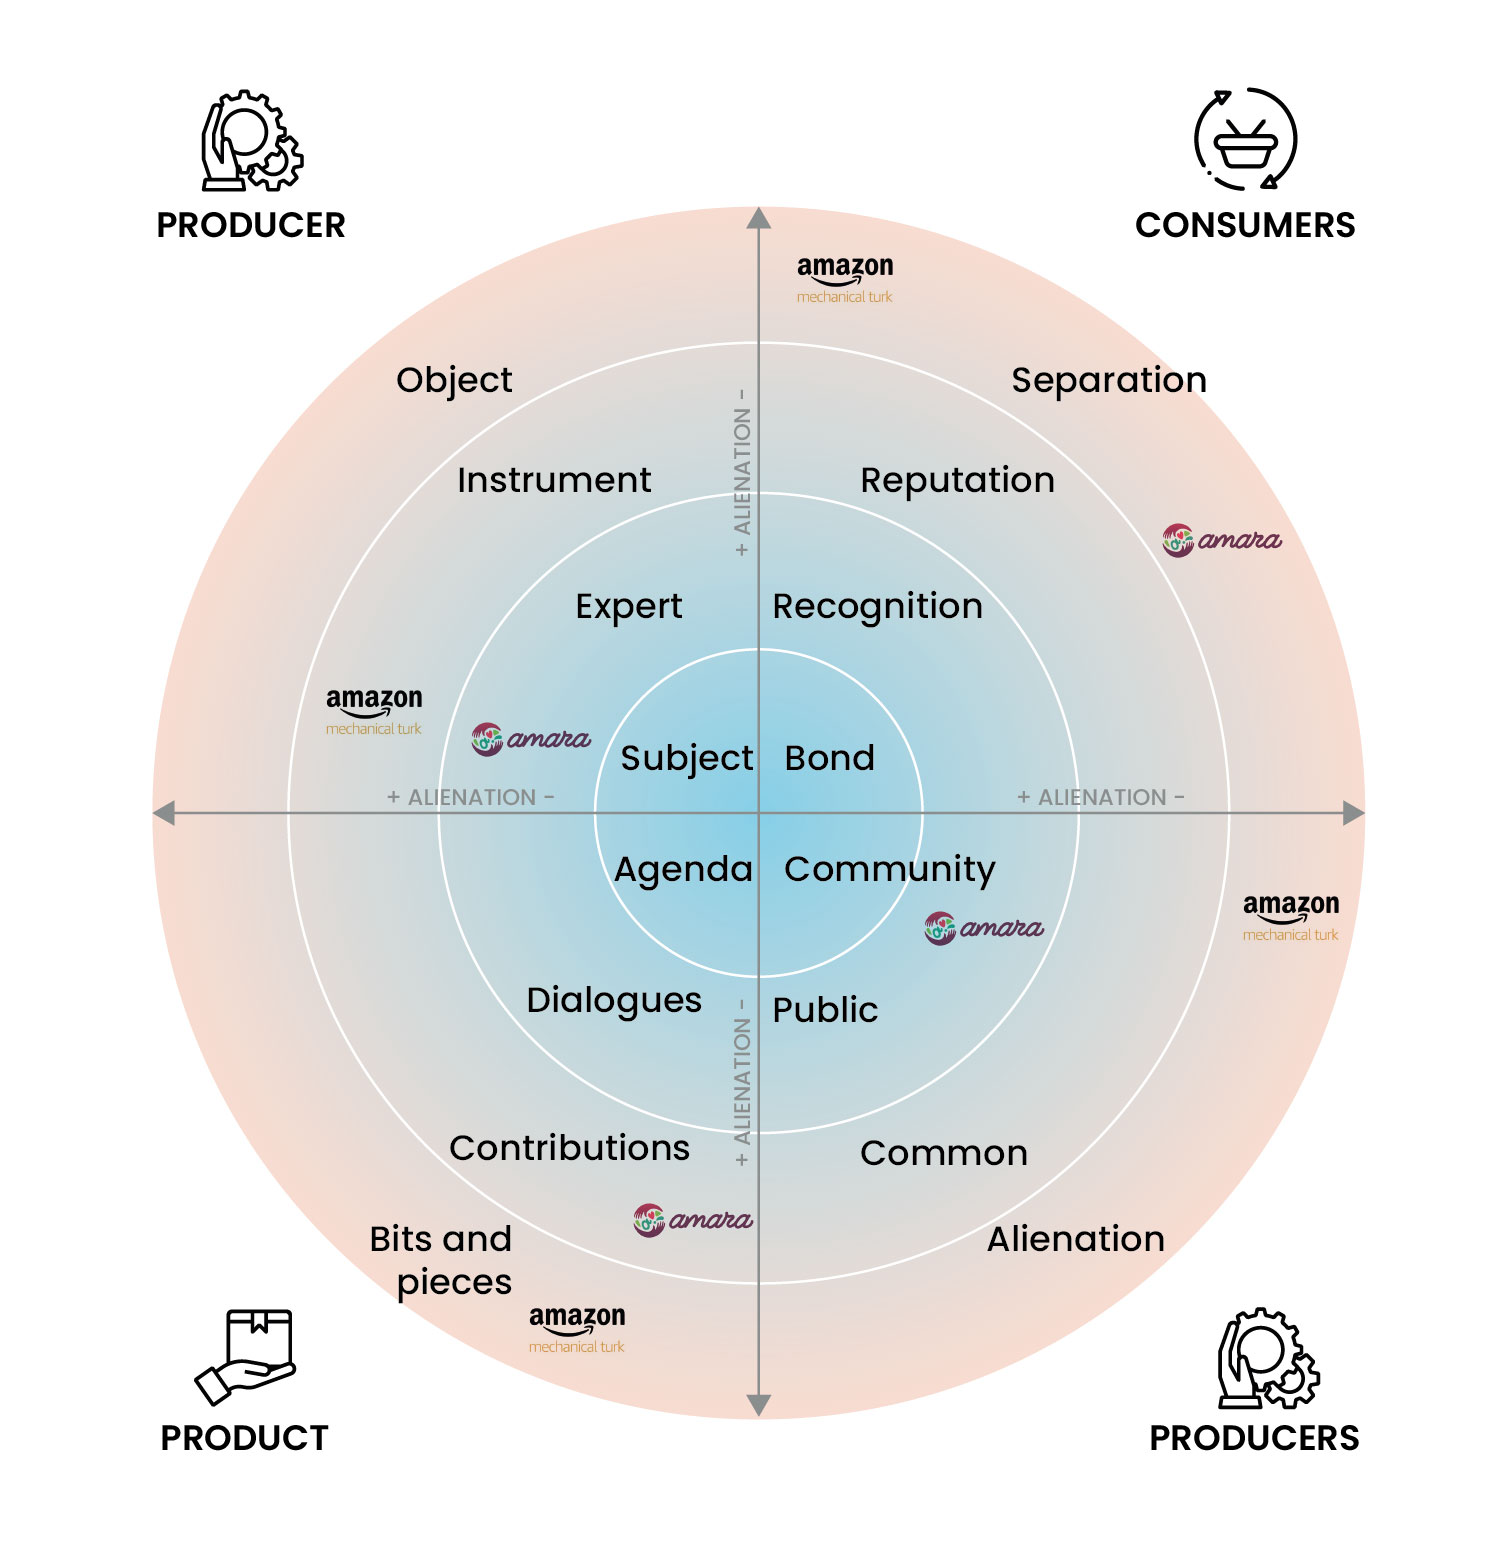
\includegraphics[width=.65\textwidth,height=.5\textheight]{figures/diagrama_02.jpg}
    \caption{A graphic representation of Hansson et al.’s \cite{hansson_capitalizing_2018} typology of alienation, according to Marx’s \cite{10.2307/2550890} four types of relationship. The further from the centre, the higher the degree of alienation. We have adapted Hansson et al.’s \cite{hansson_capitalizing_2018} Figures 1 and 2 in order to merge the categories and the position of the two key cases (from the 21 studied by them) which we employ to establish comparisons: Amara (our case study) and Amazon Mechanical Turk. See Table 4 on \cite{hansson_capitalizing_2018} for further details and a summary of the relationships with corresponding modes of productions and the categories employed.}
    \label{fig:hansson_adapted}
\end{figure}

Drawing on Hansson et al.' typology \cite{hansson_capitalizing_2018} and to further our understanding of how crowdsourcing platforms might support social relationships in these contexts, instead of merely capitalising them \cite{hansson_capitalizing_2018}, we decided to explore the following research question: \textit{can we identify alternative models for the distribution of tasks in crowdsourcing that consider the needs of the workers?}

To this aim, we establish a collaboration with Amara, whose strong cooperative values \cite{gray2019ghost} offer an opportunity to design models of task distribution in which the producer is also the owner of the means of production and the products created are an expression of self-realisation \cite{hansson_capitalizing_2018}. Since, following the concepts from Hansson et al.' typology \cite{hansson_capitalizing_2018} depicted in Figure \ref{fig:hansson_adapted}, Amara contrasts with platforms such as AMT \cite{gray2019ghost}, which understand workers as ``instruments'' from which ``bits and pieces'' can be sourced \cite{hansson_capitalizing_2018}. 

